% CQL Agreement by Distance to First Down
% Replaces: tab:cql-context-agreement in section_fourth_down_cql.tex
% Bar chart with trend showing distance-dependent agreement pattern

\begin{figure}[htbp]
\centering
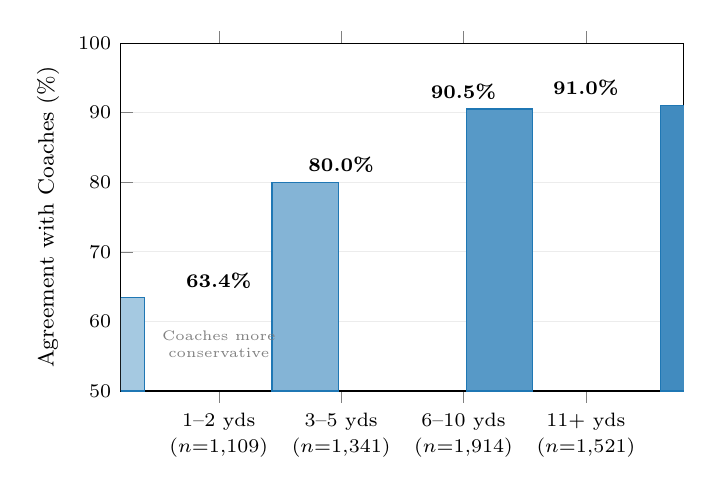
\begin{tikzpicture}
\definecolor{accent}{RGB}{31,119,180}

\begin{axis}[
  width=0.72\textwidth,
  height=6cm,
  ybar,
  bar width=24pt,
  ylabel={Agreement with Coaches (\%)},
  ylabel style={font=\footnotesize},
  ymin=50, ymax=100,
  xtick={1,2,3,4},
  xticklabels={
    {\shortstack{1--2 yds\\($n{=}1{,}109$)}},
    {\shortstack{3--5 yds\\($n{=}1{,}341$)}},
    {\shortstack{6--10 yds\\($n{=}1{,}914$)}},
    {\shortstack{11+ yds\\($n{=}1{,}521$)}}
  },
  xticklabel style={font=\scriptsize},
  ytick={50,60,70,80,90,100},
  yticklabel style={font=\scriptsize},
  grid=major,
  grid style={gray!15},
  xmajorgrids=false,
  enlarge x limits={abs=0.8},
]

% Agreement bars (gradient intensity by value)
\addplot[fill=accent!40, draw=accent] coordinates {(1, 63.39)};
\addplot[fill=accent!55, draw=accent] coordinates {(2, 80.01)};
\addplot[fill=accent!75, draw=accent] coordinates {(3, 90.54)};
\addplot[fill=accent!85, draw=accent] coordinates {(4, 90.99)};

% Value labels
\node[font=\scriptsize\bfseries, anchor=south] at (axis cs:1,63.39) {63.4\%};
\node[font=\scriptsize\bfseries, anchor=south] at (axis cs:2,80.01) {80.0\%};
\node[font=\scriptsize\bfseries, anchor=south] at (axis cs:3,90.54) {90.5\%};
\node[font=\scriptsize\bfseries, anchor=south] at (axis cs:4,90.99) {91.0\%};

% Annotation for short yardage
\node[font=\tiny, text=black!50, align=center, anchor=north] at (axis cs:1,60)
  {Coaches more\\conservative};

\end{axis}
\end{tikzpicture}
\caption[CQL distance-dependent agreement]{CQL agreement with coaching decisions by yards-to-go ($n=5{,}885$ plays, 2024). Short-yardage situations (1--2 yards, 63.4\%) show lowest agreement---where coaches are most conservative relative to expected-value-optimal play. Agreement exceeds 90\% for 6+ yard situations where punt/field goal decisions are clear.}
\label{fig:cql-distance-chart}
\end{figure}
